\section{问题二：含质量与配比的广义标度律}
\label{sec:5.3}

\subsection{问题重述}
\label{sec:5.3.1}

问题二把经典标度律扩展为同时依赖参数量 $N$、训练 token 数 $D$、B 组质量 $Q_{\rm B}$ 与领域配比 $\bp$ 的损失模型，并完成四项分析：估计各因素的边际效用与弹性；借助问题一的迁移结构讨论领域间的功能替代与覆盖互补；给出「提高质量」与「扩大参数或算力」相互替代的条件及数值例子；在附件 B 上完成参数估计、嵌套检验与留出检验，并把冻结参数交给后续问题。附件 A 仅通过问题一已输出的域质量与配比接口进入，本问直接使用附件 B。下文公式中的 $Q$ 均指 $Q_{\rm B}$。

\subsection{问题分析}
\label{sec:5.3.2}

\textbf{经典基线。} 在 B1（8 个 Pythia 模型、1,176 行）上估计 $L_0(N,D)=E+AN^{-\alpha}+BD^{-\beta}$\cite{pythia}。B1 损失与 Hoffmann 等\cite{hoffmann}的公开公式常数几乎重合，因此把其训练设定作为真实来源信息、把损失数值作为公式生成的基线。参数用幂次网格搜索、$E,A,B$ 用线性最小二乘，并用 $C/(6ND)$ 核对算力记账。

\textbf{质量项。} 题目允许采用「$Q=1$ 时退化为经典形式」一类约束，但须说明依据。本文采用该约束（$Q_{\rm B}=1$ 且取参考配比时回到 $L_0$），依据在模型建立中从刻度锚定、可识别性与嵌套检验三方面给出，并用 B6 的 $Q=1$ 切片事后检验。质量网格只出现在半合成的 B6、B7、B8，质量乘在参数项还是数据项、随质量变化的曲率如何，均由候选比较确定，且 B8 与 B6/B7 方向相反。本文在同一骨架上比较幂次、指数、线性三类乘子以及有无地板、$\kappa$ 是否可收缩的嵌套族，用 B6 训练、B7 新增点留出。主式固定为幂次 M4 加地板，把质量解释为有效参数量与有效数据量；该形状来自有效样本量的恒定弹性设定\cite{subramanyam}，而非交叉验证排名，留出误差更低的线性、指数对照一并报告。

\textbf{两套实验的统一。} 附件 A 是固定小规模的配比实验，附件 B 是规模实验，二者都以交叉熵为观测量，但没有同一批 $(N,D,Q,\bp)$ 的联合试验。配比只能通过问题一在 1M 上估计的 clr 系数乘到 B 侧可约损失上。A4/A5 全部位于 1M，无法识别配比斜率随 $N$ 的变化，因此不估计尺度项，只设两个零新增参数的强度假设，再用 A6–A11 的观测斜率作事后比较。

\textbf{边际、替代与单位算力。} 目标写成闭式后，弹性、等损失曲线与 $6ND=C$ 上的最优参数量均可解析求出并用数值解核对。领域关系取自问题一迁移矩阵行向量的余弦；单位算力比较把提质成本 $g(Q)$ 与扩参数算力放在同一 FLOP 上，回答「一份算力投向质量还是参数」。

\subsection{模型假设}
\label{sec:5.3.3}

\begin{enumerate}
\item \textbf{同一观测量。} 附件 A、B 的损失均为验证集交叉熵，可写入同一个 $L$；通过 $Q=1$ 切片与 B4、B5 的趋势相关核对。
\item \textbf{经典骨架。} 损失的规模部分取 $L_0=E+AN^{-\alpha}+BD^{-\beta}$，$\alpha,\beta>0$，$E$ 为不可约损失；B1 由公开公式生成，用拟合残差和 $C/(6ND)$ 核对。
\item \textbf{退化条件（采用的约束）。} $Q=1$ 且 $\bp=\bp_{\rm ref}$ 时质量乘子、配比乘子均为 1 且质量加项为 0，广义式回到 $L_0$。这是本文主动采用的约束而非题设给定，依据见 \ref{sec:5.3.5}「退化约束的依据」，并由 B6 的 $Q=1$ 切片检验；$\bp_{\rm ref}$ 取 A4 训练配比均值，作为 B 隐含 Pile 配比的代理。
\item \textbf{质量的两条作用通道。} 质量缺陷一方面按比例放大随规模衰减的可约损失（乘性通道，即有效规模打折），另一方面留下一项不随 $N,D$ 增大而消失的附加损失 $k_0(1-Q)$，$k_0\ge0$（加性通道，本文称为\textbf{质量地板}）。配比乘子只乘随规模衰减的两项，不乘 $E$ 与地板。两条通道的依据见 \ref{sec:5.3.5}，是否都需要由嵌套 $F$ 检验裁决。
\item \textbf{质量口径。} 主映射取 $Q_{\rm B}=Q_{\rm A}=\sum_i p_iQ_i$，推荐配比处 $Q_0=0.6624$；副映射 $Q_{\rm B}=Q_{\rm A}/Q_0$ 会使部分领域超出 $[0,1]$，仅作敏感性处理。
\item \textbf{配比强度不随规模估计。} 主假设 H$_{\rm red}$ 把配比乘在可约损失上、强度 $s_{\rm red}$ 用 1M 训练集定死，上界 H$_{\rm tot}$ 把同一偏离乘在总损失上；A6–A11 只用于事后比较，不回头改参数。
\end{enumerate}

\subsection{符号说明}
\label{sec:5.3.4}

本节符号与 \ref{sec:4} 表~\ref{tab:symbol} 一致，额外中间量为 $T_N=AN^{-\alpha}h_N(Q)$、$T_D=BD^{-\beta}h_D(Q)$、$R=T_N+T_D$ 与弹性 $\varepsilon_N,\varepsilon_D,\varepsilon_Q$，均在下一小节定义处给出。

\subsection{模型建立}
\label{sec:5.3.5}

\textbf{经典基线。} 在 B1（\texttt{N\_params\_B}/\texttt{D\_tokens\_B} 乘 $10^9$）上估计 $L_0(N,D)=E+AN^{-\alpha}+BD^{-\beta}$。$\alpha$ 在 $[0.30,0.38]$、$\beta$ 在 $[0.24,0.32]$ 按步长 $0.002$ 网格搜索，$E,A,B$ 在每格点由线性最小二乘给出，取训练误差最小者；以 $C/(6ND)$ 中位比核对算力记账（$C$ 由 \texttt{C\_FLOPs\_1e21} 乘 $10^{21}$）。

\textbf{广义标度律（主式）。} 在 $L_0$ 的可约部分上乘质量与配比因子，质量地板留在括号外：
\begin{equation*}
L(N,D,Q,\bp)=E+k_0(1-Q)+\bigl[AN^{-\alpha}Q^{-\kappa_N}+BD^{-\beta}Q^{-\kappa_D}\bigr]\exp\!\bigl(s_{\rm red}\tilde\varphi(\bp)\bigr),\quad k_0\ge0 .
\end{equation*}
该式满足三条性质：$Q=1$ 时 $\kappa$ 乘子为 1；$\kappa\ge0$ 时 $L$ 随 $Q$ 单调不增；$N,D\to\infty$ 时 $L\to E+k_0(1-Q)$，质量缺陷留下不随规模消失的地板。

\textbf{为什么乘性与加性并存。} 乘性部分刻画「一份 token、一份参数能换来多少有效学习」：低质量语料相当于打了折扣的样本，把 $D_{\rm eff}=D\,g(Q)$ 代入 $BD^{-\beta}$ 即得乘在可约项上的因子 $g(Q)^{-\beta}$，其效应随 $N,D$ 增大按同一幂律衰减。加性部分刻画规模无法消除的残余：$E$ 是评测分布自身的熵，规模趋于无穷时模型逼近的是训练分布，质量缺陷（噪声、重复、低信息文本）使训练分布偏离评测分布，这一失配不随 $N,D$ 消失；而任何乘在可约项上的因子在 $N,D\to\infty$ 时都随之趋于 0，无法表达它，只能作为 $E$ 之外的加项，并取在 $Q=1$ 处为零的一阶形式 $k_0(1-Q)$。数据同时拒绝两种单一通道：纯加性（M0＋地板）意味着质量收益与规模无关，但质量总收益与 $\ln N$ 的相关系数为 $-0.767$，其留一规模 CV 为 $0.0781$，高于主式的 $0.0598$；纯乘性（M4 去地板）留出 RMSE 升至 $0.0839$，嵌套检验中地板 $F=307.11$；附加 $(1-Q)^2$ 项不显著（$p=0.195$），一阶形式已足够（表~\ref{tab:q2form}）。配比乘子沿用主假设 H$_{\rm red}$ 只作用于可约项，$E$ 与地板作为规模极限不设配比作用，其上界情景 H$_{\rm tot}$ 见 \ref{sec:5.3.7}。

\textbf{乘子形状。} 幂次形状来自有效样本量视角\cite{subramanyam}，与数据受限标度律中「有效数据量」的处理一致\cite{muennighoff}：设质量为 $Q$ 的语料在信息上等价于 $D_{\rm eff}=D\,g(Q)$ 个理想质量 token，$g$ 单调不减且 $g(1)=1$。若再设质量的作用具有恒定弹性，即 $\mathrm d\ln g/\mathrm d\ln Q=\gamma$ 不随 $Q$ 变化，则唯一解为 $g(Q)=Q^{\gamma}$，数据项化为 $BD^{-\beta}Q^{-\gamma\beta}$，即幂次乘子 $Q^{-\kappa_D}$（$\kappa_D=\gamma\beta$），参数侧同理。恒定弹性与标度律本身的幂律结构一致，并给出 $g(0)=0$，即不含信息的语料不贡献有效样本；线性与指数乘子在 $Q\to0$ 时仍保留正的有效规模，没有这一边界含义。这是建模设定而非由数据推出，其留出误差代价在 \ref{sec:5.3.7} 与线性、指数对照并列报告。由此定义有效规模
\begin{equation*}
N_{\rm eff}=N\,Q^{\kappa_N/\alpha},\qquad D_{\rm eff}=D\,Q^{\kappa_D/\beta}.
\end{equation*}

配比标量来自问题一 1M 的 clr 系数并在 $\bp_{\rm ref}$ 归一：
\begin{equation*}
\varphi(\bp)=\frac1{13}\sum_{v=1}^{13}\boldsymbol\beta_v^{(1{\rm M})}\cdot\operatorname{clr}(\bp),\qquad
\tilde\varphi(\bp)=\varphi(\bp)-\varphi(\bp_{\rm ref}),\qquad \bp_{\rm ref}=\text{A4 训练配比均值}.
\end{equation*}
$Q=1$、$\bp=\bp_{\rm ref}$ 时两个乘子均为 1、地板为 0，式退化为 $L_0$。

\textbf{退化约束的依据。} 题目未强制该约束，本文采用它的理由有三。其一，刻度锚定：B1 不含质量变量，是在固定语料与固定配比下测得的经典律，本身就是「质量与配比不变」的切片；令 $Q_{\rm B}=1$、$\bp=\bp_{\rm ref}$ 对应这一切片，等于把 B 组质量刻度的上端锚定在 B1 基线上。其二，可识别性：质量乘子只以 $A\,h_N(Q)$、$B\,h_D(Q)$ 的乘积形式出现，常数因子可在两者之间任意转移，地板常数也会与 $E$ 混淆，必须在某一质量处归一；取 $h(1)=1$、地板在 $Q=1$ 为零，使 $E,A,B,\alpha,\beta$ 保留 B1 上的经典含义，质量参数只描述相对理想质量的偏离，配比取 $\bp_{\rm ref}$ 归一同理。其三，可检验性：经典式成为嵌套零模型 M0，质量项的每个自由度都可用 $F$ 检验判断是否必要。该约束是否被数据接受由事后检验回答：B6 中 $Q=1$ 的 45 点相对 B1 拟合的 $L_0$ 平均残差 $+0.0036$，$95\%$ 区间 $[-0.0120,0.0193]$ 含 0（\ref{sec:5.3.7}）。需要说明，这一锚定只在 B 组刻度上成立；A 组质量能否等同于 B 组质量由假设 5 的质量口径单独承担，并以副映射作敏感性分析。

\textbf{嵌套候选族。} 每种乘子形状（幂次 $Q^{-\kappa}$、指数 $e^{\kappa(1-Q)}$、线性 $1+\kappa(1-Q)$）下比较 M0（$\kappa_N=\kappa_D=0$）、M1（$\kappa_N=0$）、M2（$\kappa_D=0$）、M3（$\kappa_N=\kappa_D$）、M4（两项各一个 $\kappa$），再交叉有无地板，共 26 个候选。$\kappa$ 在 $[0,\kappa_{\max}]$ 上网格加密最小二乘（幂次/指数为 $1.2$、线性为 $3.0$），$k_0$ 在每个 $\kappa$ 上闭式求出并截断为非负。

\textbf{训练与留出边界。} 只用 B6 的 360 点估计参数、比较候选；B6 的 360 点全部出现在 B7 且同点损失相同，B7 中不在 B6 的 90 点（全部 $Q=0.5,0.7$、覆盖 45 个 $(N,D)$ 格）作留出，按 $Q,N,D$ 分组报告 RMSE 与残差；全 B7 450 点的拟合含训练点，仅作对照（\texttt{fullB7\_comparison}）。主式固定为幂次 M4 加地板；交叉验证规则选出的线性 M4+F 仅写入 \texttt{cv\_rule\_choice}，不决定主式。

\textbf{配比通道。} A4/A5 全在 1M，无法识别配比效应随 $N$ 的变化，故只设两个零新增参数假设：H$_{\rm red}$（主）令配比乘可约部分、强度恒定，$s_{\rm red}=c_{\rm train}/\sigma_{\rm train}$；H$_{\rm tot}$（上界）令配比乘总损失。两假设参数只用 1M 训练行确定，A6–A11 只以冻结系数计算校准斜率作事后比较。

\textbf{边际、弹性与替代闭式。} 记 $T_N=AN^{-\alpha}Q^{-\kappa_N}$、$T_D=BD^{-\beta}Q^{-\kappa_D}$，令配比乘子暂为 1：
\begin{equation*}
\frac{\partial L}{\partial Q}=-\frac{\kappa_NT_N+\kappa_DT_D}{Q}-k_0,\qquad
\varepsilon_N=-\frac{\alpha T_N}{L},\quad \varepsilon_D=-\frac{\beta T_D}{L},\quad \varepsilon_Q=\frac{Q}{L}\frac{\partial L}{\partial Q}.
\end{equation*}
固定 $D$ 把质量由 $Q$ 提到 $Q'$，若只靠增大 $N$ 拉回损失，则
\begin{equation*}
t=\Bigl(\frac{Q}{Q'}\Bigr)^{\kappa_N}+\frac{T_D}{T_N}\left[\Bigl(\frac{Q}{Q'}\Bigr)^{\kappa_D}-1\right]-\frac{k_0(Q'-Q)}{T_N},\qquad N'=N\,t^{-1/\alpha},
\end{equation*}
$t>0$ 时该式给出所需参数倍数，$t\le0$ 时任何有限参数都补不回这次提质。在 $6ND=C$、配比乘子为 1 时，最优参数与地板无关：
\begin{equation*}
N^*(C,Q)=\left(\frac{\alpha A Q^{-\kappa_N}}{\beta B Q^{-\kappa_D}}\right)^{1/(\alpha+\beta)}
\left(\frac{C}{6}\right)^{\beta/(\alpha+\beta)},\qquad D^*=\frac{C}{6N^*}.
\end{equation*}
$\kappa_N>\kappa_D$ 时质量越低、$N^*$ 越大。沿最优前沿，质量由 $Q$ 提到 $Q'$ 等效于算力乘以
\begin{equation*}
M=\left\{\frac{R^*(C,Q')-k_0(Q'-Q)}{R^*(C,Q)}\right\}^{-1/a},\qquad
a=\frac{\alpha\beta}{\alpha+\beta},\quad R^*=L^*-E-k_0(1-Q),
\end{equation*}
花括号内不大于 0 时再大算力也追不上。$k_0=0$ 时 $M$ 与 $C$ 无关，$k_0>0$ 时 $M$ 随预算上升。

\textbf{单位算力取舍与领域关系。} 单位算力收益 $\mathrm{MU}_x=-(\partial L/\partial x)\div(\partial C/\partial x)$，总成本取
\begin{equation*}
C=(6+\eta L_{ctx})ND+D\,[g(Q)-g(Q_0)]_+,\qquad \eta=2\times10^{-4},\;L_{ctx}=2048,
\end{equation*}
与问题三共用同一成本口径。配比边际 $\partial L/\partial p_i=s_{\rm red}R\,\partial\varphi/\partial p_i$。领域关系由迁移矩阵行向量余弦定义：余弦 $>0.7$ 记功能替代、$<-0.3$ 记覆盖互补；线性 clr 模型无交互项，超可加意义的互补不可识别。

\subsection{模型求解}
\label{sec:5.3.6}

本问使用 Python 3.12.7、NumPy 1.26.4、pandas 2.2.2、SciPy 1.13.1，随机种子 $2026$，脚本为 \texttt{q2\_01\_fit.py}、\texttt{q2\_02\_theory.py}、\texttt{q2\_03\_economics.py}，只读问题一接口、不读附件 A 原始表与缓存。$\alpha,\beta$ 网格搜索、$E,A,B$ 线性最小二乘；质量参数 $\kappa$ 在 $[0,1.2]$（线性对照到 $3.0$）以步长 $0.02$ 搜索并在最优点两侧加密两轮，$k_0$ 闭式求出并截断非负；参数区间用 B1 行重抽样与 B6 $(N,D)$ 格簇重抽样各 300 次，$\alpha,\beta$ 固定。闭式结果与数值解逐项对照。

\subsection{结果分析}
\label{sec:5.3.7}

\textbf{经典基线。} B1 拟合结果为 $E=1.6901$、$A=406.39$、$\alpha=0.34$、$B=410.59$、$\beta=0.28$，训练 RMSE 为 $1.51\times10^{-4}$，对 Hoffmann 常数的 RMSE 为 $1.65\times10^{-4}$，$C/(6ND)$ 中位比为 $1.0000$（\texttt{T20\_baseline\_fit.csv}），与公开公式吻合到 $10^{-4}$ 量级，是可靠的基线锚点。

\textbf{质量参数与留出表现。} 主式参数为 $\kappa_N=0.1416$、$\kappa_D=0.0112$、$k_0=0.2280$，$95\%$ 区间分别为 $[0.1264,0.1568]$、$[0.0000,0.0408]$、$[0.2013,0.2554]$，且 $P(\kappa_N>\kappa_D)=P(k_0>0)=1$（\texttt{T22\_params\_ci.csv}、\texttt{P2\_bootstrap.npz}）。嵌套检验中地板被强烈支持（$F=307.11$，$p<10^{-15}$），$\kappa_N=\kappa_D$ 被拒绝（$F=57.19$，$p=3.4\times10^{-13}$），而 $\kappa_D=0$ 不能拒绝（$F=0.63$，$p=0.43$），数据侧质量幂次较弱，主式仍按 M4 保留该项（\texttt{T21b\_nested\_tests.csv}）。

候选形式的比较与留出表现见表~\ref{tab:q2form}。B7 新增 90 点上，主式留出 RMSE 为 $0.0531$（平均偏差 $-0.0219$），按 $Q$ 分组为 $0.0538$（$Q=0.5$）与 $0.0525$（$Q=0.7$），按规模分组以 70M 的 $0.0865$ 最大；格内噪声代理为 $0.0458$。交叉验证选出的线性 M4+地板留出 RMSE 为 $0.0416$，比主式低约 $22\%$。需说明两点：一是主式与线性、指数对照（$0.0421$）的留出 RMSE 都与噪声代理同量级，与线性的差值 $0.0115$ 约为噪声代理的四分之一；二是留出点只位于 $Q=0.5,0.7$ 两档内部，只能检验插值精度，无法区分三种形状在 $Q\to0$ 与 $Q\to1$ 边界上的差异，而有效规模的解释和问题三中 $D^*/N^*$ 随 $Q$ 的幂律关系恰依赖这一部分。因此本文保留幂次主式，以约 $0.01$ 的留出误差换取有效规模的解释与边界含义，线性、指数对照作为稳健性参照并列报告。

\begin{table}[H]
\centering\small
\caption{质量项候选比较（B6 训练，留出为 B7 新增 90 点；源自 \texttt{T21\_form\_selection.csv}）}
\label{tab:q2form}
\begin{tabularx}{\textwidth}{@{}lllrrr@{}}
\toprule
形状 & 模型 & $\kappa_N,\kappa_D,k_0$ & 留一规模 CV & 留出 RMSE & 留出偏差 \\
\midrule
— & M0 & $0,0,0$ & 0.2100 & 0.1616 & $-0.146$ \\
— & M0＋地板 & $0,0,0.363$ & 0.0781 & 0.0595 & $-0.001$ \\
幂次 & M4（去地板） & $0.203,0.153,0$ & 0.0813 & 0.0839 & $-0.070$ \\
\textbf{幂次} & \textbf{M4＋地板（主）} & $\mathbf{0.142,0.011,0.228}$ & \textbf{0.05979} & \textbf{0.0531} & $\mathbf{-0.022}$ \\
指数 & M4＋地板 & $0.370,0.131,0.144$ & 0.05324 & 0.0421 & $-0.005$ \\
线性 & M4＋地板（CV 对照） & $0.430,0.139,0.142$ & 0.05321 & 0.0416 & $-0.001$ \\
\bottomrule
\end{tabularx}
\end{table}

\begin{figure}[H]
\centering
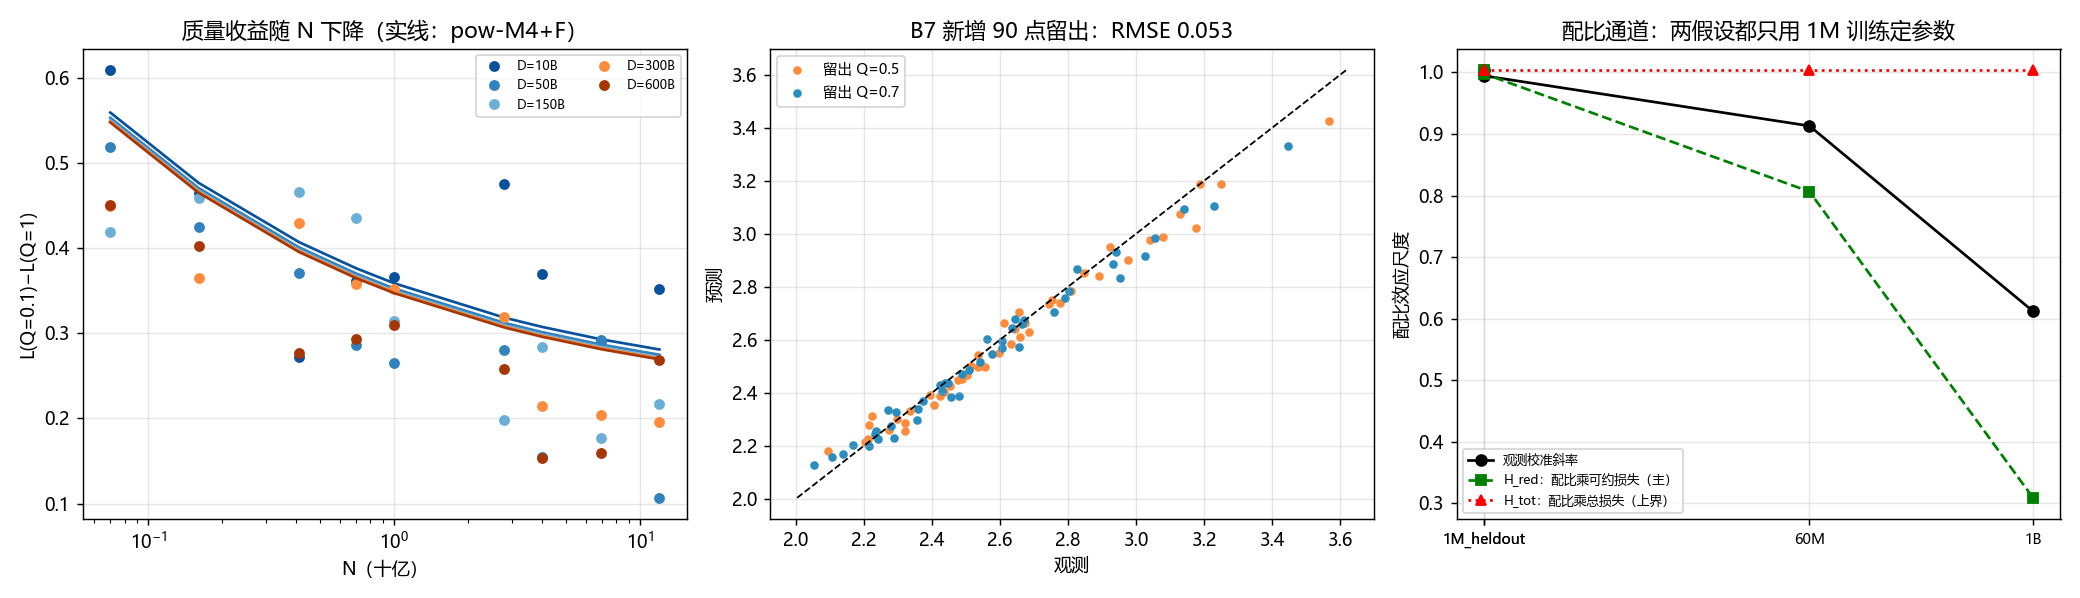
\includegraphics[width=\textwidth]{figs/q2_F22_form_selection.png}
\caption{质量项候选比较与 B7 新增 90 点的留出表现}
\label{fig:F22_form_selection}
\end{figure}

退化约束的事后检验：B6 中 $Q=1$ 的 45 点相对 $L_0$ 平均残差为 $+0.0036$、$95\%$ 区间 $[-0.0120,0.0193]$；附加 $(1-Q)^2$ 项不显著（$p=0.195$）。质量总收益 $\Delta L$（$Q$ 由 $0.1$ 到 $1$）范围为 $[0.107,0.609]$，与 $\ln N$ 相关 $-0.767$，质量收益随参数规模变小，与 $\kappa_N>\kappa_D$ 方向一致（\texttt{T21c}、\texttt{T21d}）。B8 在最低质量档平均损失仅 $0.545$、$64.26\%$ 的点低于 $E$，方向相反，不并入拟合（\texttt{T21e}）。

\textbf{边际效用与弹性。} 在 $N=10^9$、$D=3\times10^{11}$、$Q=Q_0$ 处损失 $L=2.3945$，三弹性为 $\varepsilon_N=-0.0533$、$\varepsilon_D=-0.0295$、$\varepsilon_Q=-0.0865$，质量弹性约为参数弹性的 $1.62$ 倍（其中 $72.97\%$ 来自地板）；四个配比份额的弹性和仅 $0.0072$。规模越大、质量越敏感：在 $(10^{10},10^{12})$ 与 $(7\times10^{10},2\times10^{12})$、$Q=0.9$ 处 $\varepsilon_Q/\varepsilon_N$ 升至 $4.13$、$7.60$，地板占质量导数的 $89.04\%$、$93.76\%$（\texttt{T26\_elasticities.csv}、\texttt{T31}）。

\textbf{质量—参数替代。} 固定 $D=3\times10^{11}$，质量提高 $0.1$ 的等效参数倍数见表~\ref{tab:q2sub}：模型越大、同样提质越难用堆参数补回；千亿参数处约需 $3$ 倍参数，而去地板后降到 $1.3$–$1.5$，凸显地板只能靠提质消除。

\begin{table}[H]
\centering\small
\caption{质量提高 0.1 的等效参数倍数（固定 $D=3\times10^{11}$；括号内为去地板对照；源自 \texttt{T24\_equiv\_substitution.csv}）}
\label{tab:q2sub}
\begin{tabularx}{\textwidth}{@{}lccc@{}}
\toprule
起点 $Q$ & $N=10^9$ & $N=10^{10}$ & $N=10^{11}$ \\
\midrule
0.5$\to$0.6 & 1.299 (1.182) & 1.648 (1.268) & 2.996 (1.488) \\
0.7$\to$0.8 & 1.282 (1.130) & 1.641 (1.190) & 3.066 (1.337) \\
0.9$\to$1.0 & 1.274 (1.102) & 1.644 (1.148) & 3.144 (1.258) \\
\bottomrule
\end{tabularx}
\end{table}

\textbf{质量—算力替代。} 沿算力前沿，质量由 $0.7$ 提到 $0.8$ 等效于算力乘 $1.191/1.485/2.134$（$C=10^{19}/10^{22}/10^{24}$），无地板时恒为 $1.165$；$Q=0.5$ 的 $N^*$ 比 $Q=1$ 大 $15.7\%$，$C=10^{24}$、$Q=0.5$ 时地板占可约损失 $32.94\%$（\texttt{T25}、\texttt{T27}、\texttt{T29}，图~\ref{fig:F21_theory}）。高预算端的倍数与地板份额含外推成分，按假设使用。

\begin{figure}[H]
\centering
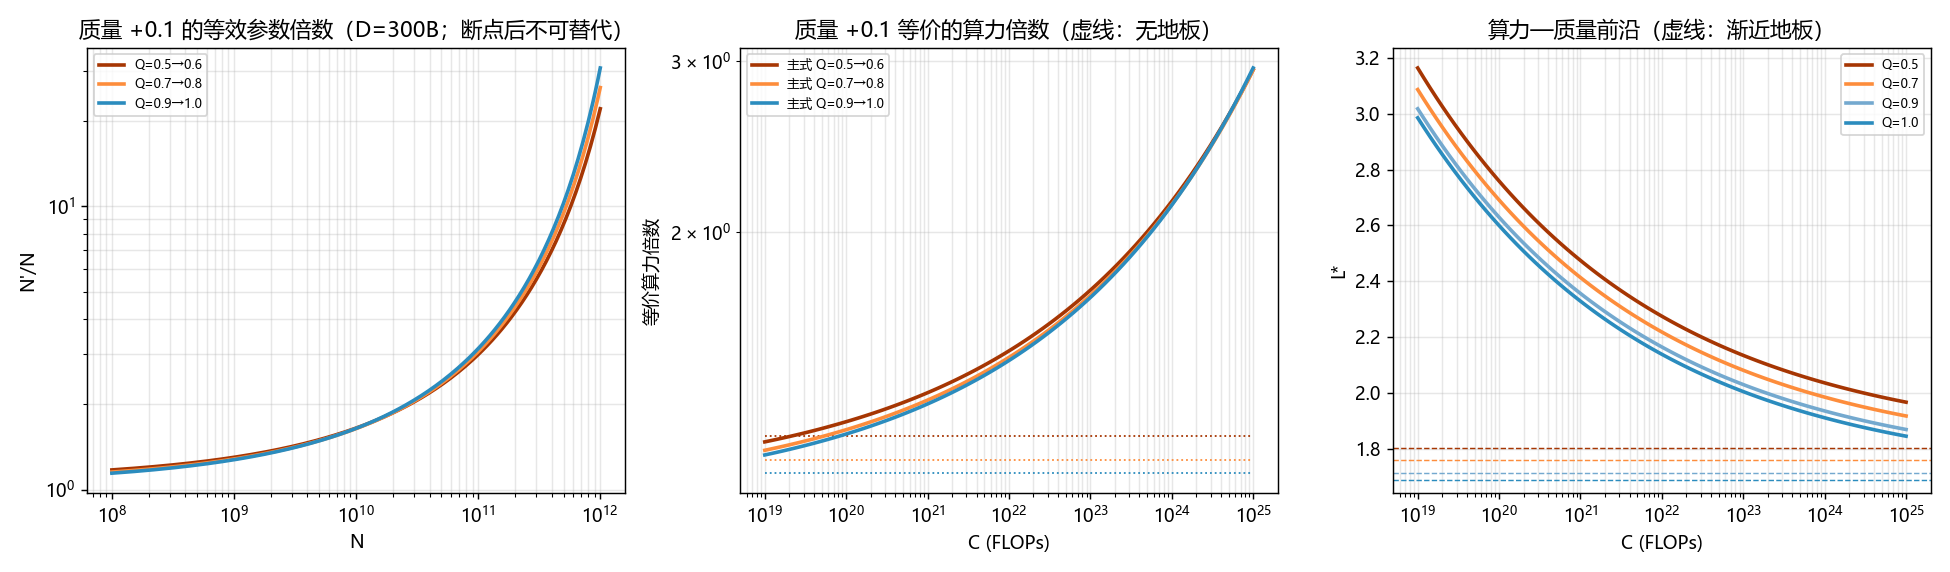
\includegraphics[width=\textwidth]{figs/q2_F21_theory.png}
\caption{等效参数倍数、等价算力倍数随预算变化与算力—质量前沿}
\label{fig:F21_theory}
\end{figure}

\textbf{单位算力取舍。} 表~\ref{tab:q2mu} 给出 $\mathrm{MU}_Q/\mathrm{MU}_N$：比值大于 1 表示一份算力用于提质更有效。$C=10^{19}$ 时指数型、幂函数型小于 1（应扩参数），对数型略大于 1；自 $C=10^{20}$ 起三种成本函数下比值均大于 1（$3.10/1.70/3.77$）并随预算迅速增大。提质更划算的质量上界在 $C=10^{19}$ 时为 $0.64/0.53/0.99$，即低预算下质量已较高时应转回扩参数。整体规律是：低预算结论对成本函数形式敏感，高预算结论稳健。

\begin{table}[H]
\centering\footnotesize
\caption{$\mathrm{MU}_Q/\mathrm{MU}_N$（$Q=Q_0$、$L_{ctx}=2048$；括号内去地板；源自 \texttt{T33}、\texttt{T33b}）}
\label{tab:q2mu}
\begin{tabularx}{\textwidth}{@{}lccc@{}}
\toprule
预算 $C$ & 指数型 & 幂函数型 & 对数型 \\
\midrule
$10^{19}$ & 0.868 (0.793) & 0.477 (0.436) & 1.057 (0.965) \\
$10^{20}$ & 3.10 & 1.70 & 3.77 \\
$10^{22}$ & 42.48 (17.95) & 23.34 (9.86) & 51.71 (21.85) \\
$10^{24}$ & 627.30 (143.65) & 344.59 (78.91) & 763.61 (174.87) \\
\bottomrule
\end{tabularx}
\end{table}

\begin{figure}[H]
\centering
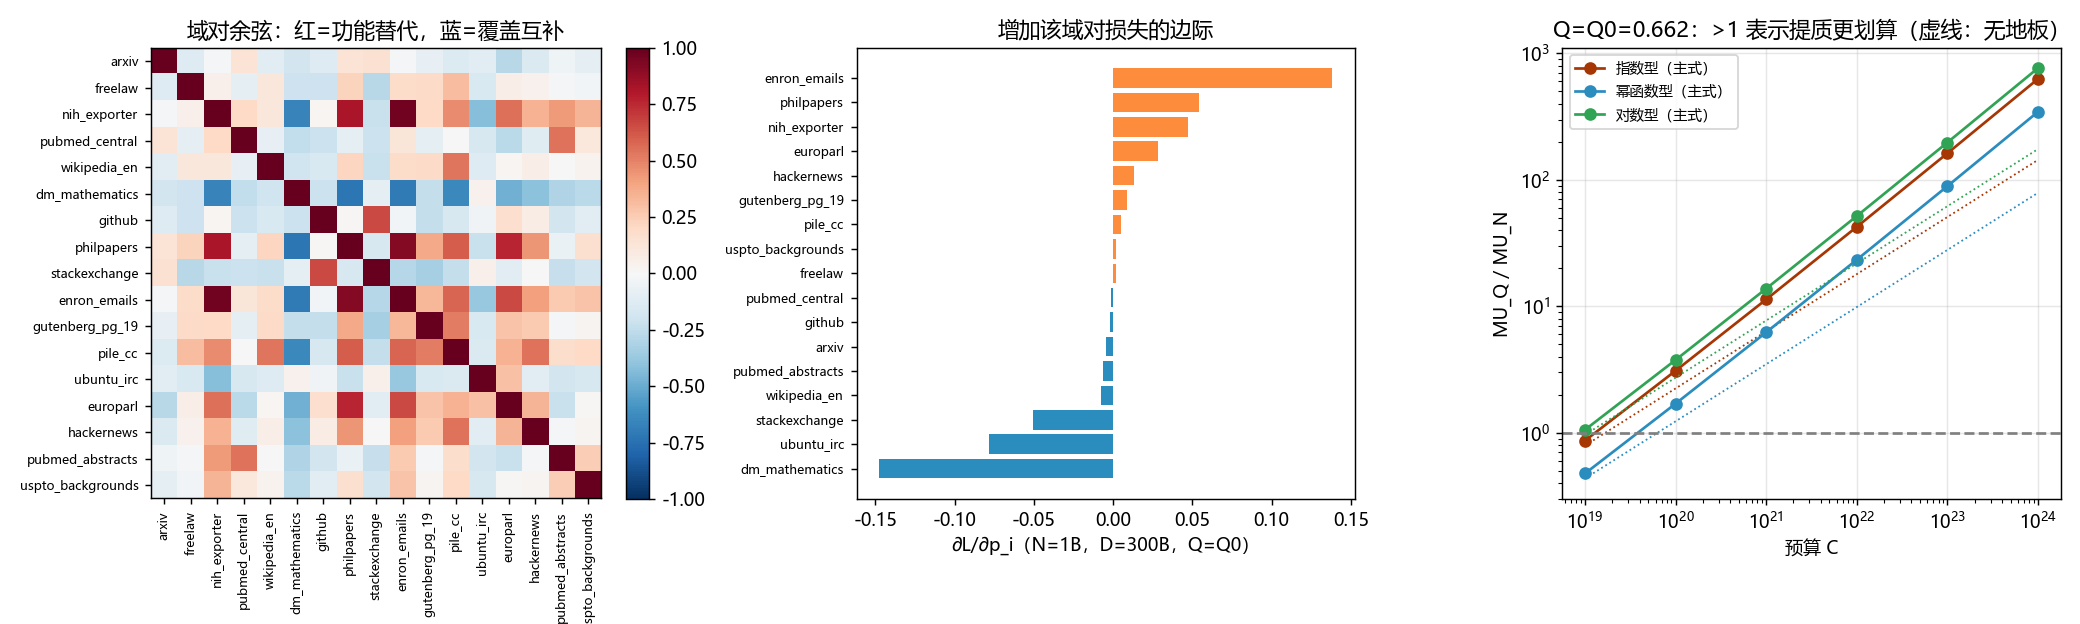
\includegraphics[width=\textwidth]{figs/q2_F23_economics.png}
\caption{域对余弦热力图、份额边际与 $\mathrm{MU}_Q/\mathrm{MU}_N$ 随预算变化}
\label{fig:F23_economics}
\end{figure}

\textbf{领域关系。} 按迁移矩阵行向量余弦，17 域对中功能替代 4 对（最强 nih\_exporter–enron\_emails，$0.969$）、覆盖互补 10 对（最强 dm\_mathematics–philpapers，$-0.725$），其余 122 对弱相关（\texttt{T32b}）。把份额拨向 dm\_mathematics 使等权损失下降最快（$\partial L/\partial p=-0.1475$），拨向 enron\_emails 上升最快（$+0.1381$）（\texttt{T31b}）。

\textbf{配比通道的位置。} 通道参数为 $c_{\rm train}=1.0039$、$Q_{\rm ref}=0.6640$、$\sigma_{\rm train}=0.6694$，故 $s_{\rm red}=1.500$；$\tilde\varphi(\bp^*)=-0.07104$、$\tilde\varphi(\text{均匀})=+0.03611$，推荐配比处乘子约为 $0.899$。表~\ref{tab:q2pchannel} 显示，60M、1B 上的观测斜率落在 H$_{\rm red}$ 与 H$_{\rm tot}$ 两个预设值之间，构成已评估点上的情景包络，为下游提供配比敏感性的下、上情景。

\begin{table}[H]
\centering\small
\caption{两个配比通道假设与观测校准斜率对照（源自 \texttt{T28\_p\_channel.csv}）}
\label{tab:q2pchannel}
\begin{tabularx}{\textwidth}{@{}l c c c c@{}}
\toprule
尺度 & 观测斜率（评估） & H$_{\rm red}$ & H$_{\rm tot}$ & 相对位置 \\
\midrule
1M 训练 & 1.004 & 1.004 & 1.004 & — \\
1M 留出 & 0.995 & 0.998 & 1.004 & — \\
60M & 0.913 & 0.807 & 1.004 & 0.540 \\
1B & 0.612 & 0.309 & 1.004 & 0.436 \\
\bottomrule
\end{tabularx}
\end{table}

\subsection{模型检验}
\label{sec:5.3.8}

\textbf{留出与嵌套。} B7 新增 90 点作 $Q$ 方向插值留出，主式留出 RMSE（$0.0531$）与噪声代理（$0.0458$）同量级，略高于线性对照（$0.0416$）。由于留出点只在 $Q=0.5,0.7$ 内部，该检验只判断插值精度，形状由有效规模设定决定（\ref{sec:5.3.5}）。地板、$\kappa_D=0$、$\kappa_N=\kappa_D$ 三个嵌套假设由 $F$ 检验裁决；$Q=1$ 切片残差区间含 0，退化约束未被数据拒绝。

\textbf{跨来源对照。} 各对照均在 $Q=1$ 切片上检查趋势：B2（半合成，$n=1{,}029$）Spearman $0.788$、偏差 $+1.178$；B3 为 B1 插值派生；B4 共 57 点、剔除 13 个近邻后 44 点 Spearman $0.975$、偏差 $+0.176$；B5 的 44 点 Spearman $0.959$；B9/B10 对齐 128 对，B10 与公式高相关是估算构造所致（\texttt{T23} 系列）。这些对照核对了趋势的一致性，B2、B3、B10 不构成质量项可泛化到真实训练的证据。

\textbf{来源审计与解析互验。} B11/B12 确认 B1 的 8 个名义规模、每模型 147 步均被检查点记录覆盖，$D/(\text{steps}\times\text{batch})$ 中位比 $0.9986$；B11 仅覆盖 3/12 模型族（\texttt{T23e}、\texttt{T23f}）。由此确认 B1 训练设定有来源记录，损失值按公开公式生成。替代条件、$N^*$ 与算力倍数的解析值与数值解误差小于 $10^{-8}$（替代倍数小于 $10^{-13}$）。

\subsection{评价与改进}
\label{sec:5.3.9}

本问主式在 $Q=1$、$\bp=\bp_{\rm ref}$ 时回到经典式，把「提质能否被规模替代」写成 $t>0$ 的可计算条件，并把 B6 拟合、B7 插值留出、跨源对照与来源审计分层报告。局限在于：质量参数来自最大约 12B 的半合成网格，高预算端地板份额与「提质远比扩参数划算」含外推成分；幂次形状来自恒定弹性的建模设定，线性、指数的留出误差低约 $0.01$，现有留出又无法检验 $Q$ 边界处的形状差异；$\kappa_D$ 较弱；$\bp_{\rm ref}$ 与恒定配比强度属建模假设。若后续取得真实跨质量训练日志，可替换 B6 重估参数并允许配比强度随 $\log N$ 变化。问题三已按幂次乘子重跑（\ref{sec:5.4}），问题四按 $Q=1$ 切片使用。
